\documentclass[../main.tex]{subfiles}

\begin{document}
\subsection{The reactive manifesto}

As mentioned in the introduction, all 
systems nowadays have to handle big amounts of data, coming from thousands of
concurrent users, which are demanding low latency responses in the order of
% by terms of -- No he encontrado esta expresión
milliseconds and robust systems with a 100\% of up time.


The reactive manifesto \autocite{2014TheManifesto} calls Reactive Systems the
ones able to cope with this expectances and gives this description: ``Reactive
Systems are more flexible, loosely-coupled and scalable. This makes them easier
to develop and amenable to change. They are significantly more tolerant of
failure and when failure does occur they meet it with elegance rather than
disaster. Reactive Systems are highly responsive, giving users effective
interactive feedback.''

%% Consider talking about https://www.lightbend.com/blog/why-do-we-need-a-reactive-manifesto

At the same time it describes what the traits of reactive systems are. 
% para este párrafo, no acabo de entender su redacción
% desde aquí
This
traits can be categorised hierarchically by the end goal they serve. Being
responsiveness the trait which directly provides value to systems and the other
three characteristics that reactive systems need to meet in order to be
responsive. 
% hasta aquí
This relationship can be visualised in the Figure
\ref{fig:reactive}.

\begin{figure}[ht] \centering
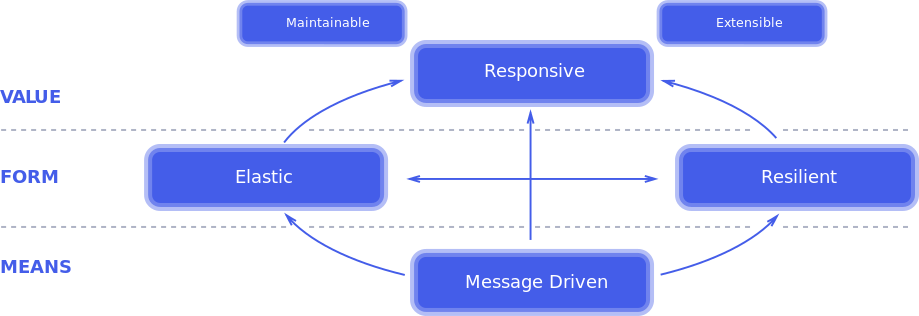
\includegraphics[width=\textwidth]{images/reactive-traits.png}
    \caption{A hierarchical view of the reactive principles.}
    \label{fig:reactive}
\end{figure}

\subsection{The reactive principles}
\subsubsection{Responsive}

Responsiveness is the cornerstone of the reactive
systems. Systems which are responsive are more comfortable to use for users as
they respond faster and adapt quicker to their needs.

Google found out in 2007 that additional 0.5 seconds of load time of a search
could lead to a loss of interest of on the search of a 20\%. \autocite{MayerGoogleYouTube}.

More recently, in an study developed by Akamai Technologies in 2017 \autocite{Akamai2017TheAkamai}, other
insights about consequences of pages responsiveness were analyzed, being some of the most
interesting the following ones:

\begin{itemize}
    \item A 100-millisecond delay in website load time can hurt conversion rates
by 7 percent.
% a qué te refieres con "conversion rates"?

    \item A two-second delay in web page load time increases bounce rates by 103
percent.

    \item 53 percent of mobile site visitors will leave a page that takes longer
than three seconds to load.
\end{itemize}

When time is that relevant in consumer satisfaction and hundred of milliseconds
makes the difference for a potential new user, it is important to design systems
that respond to user requests with low latency in a consistent manner.

\subsubsection{Resilient}

Resilience provides a better responsiveness as systems
react better to failure. A resilient system is able to operate even if parts of
it are failing. As an example, if a user is using a social network, he should be
able to see friends' posts even if the chat system is unavailable.

At the same time, resilience is the ability to recover from errors without manual
intervention meaning that local errors shouldn't be propagated but rather handled and
managed by different parts of the system.

When designing reactive systems, errors should be expected to occur. Even if all
the possible applications errors under control of the designers could be avoided, there
are other elements of the application which are out of control, such as network
errors or interactions with external systems. This principle is stated in the
\textit{Design for failure} approach \autocite{Sussna2015DesigningDelivery} which embraces the
acknowledge of possible errors, thus having to make systems which can have
errors but can gracefully recover from them.

\subsubsection{Elastic}

Applications traffic isn't stable. Online commerces usually have much higher
demands on holidays seasons like Christmas. A marketing campaign can create
higher traffic than usual in applications. Even an unexpected reference in a
newspaper or a website may increase the number of users to an unmanageable
amount for the original design.

Load balancers or more advanced orchestration systems like Kubernetes
\cite{Production-GradeKubernetes} can handle elasticity on the infrastructure
level, allowing replicas of the application to coexist. However, applications
have to be designed to allow for the distribution of work among the instances of the
application. This is referred as to Systems scalability.

\paragraph{Scalability}

The Scalability of a system is the capacity that it has to increase its
throughput respectively to its hardware resources. It is defined by the
Universal Law of Computational Scalability \autocite{Gunther2008AFunctions}, the formula
is a variation of the Amhdalh's law \autocite{Rodgers1985ImprovementsDesign} and is present in figure \ref{fig:scalability}

\begin{figure}[ht] \centering
  $C(N)={\frac {N}{1+\alpha (N-1)+\beta N(N-1)}}$
  \caption{The Universal Law of Computational Scalability formula.}
  \label{fig:scalability}
\end{figure}

In the formula, parameter $N$ represents the amount of concurrent processes
running the application, $\alpha$ is the time that is lost because of the need
to wait for shared resources to become available and $\beta$ is the time that
distributed nodes take to have consistent data.

The mere act of increasing the parallelism of an application by adding more
computation nodes doesn't mean that the application will scale linearly with it.
Systems have to be designed in order to use efficiently available computing resources.
In the Universal Law of Computational Scalability this is measured by $\alpha$
and $\beta$. If systems are not designed to be scalable both parameters will
be very high and adding parallelism can even decrease performance.

\subsubsection{Message driven}

The way to achieve Elastic and Resilient systems is by the use of asynchronous
message passing. Thanks to this mechanism application are decoupled both with respect to
their space and and time constraints.


If modules of the application communicate by means of asynchronous messages, the end
location of the resource which will handle the message is transparent for the
caller. A message will be delivered to a mailbox. The specific receptor of the
message is not known. A load balancer can choose which system will be the recipient
of the message, allowing for \textbf{Elasticity}.

As messages are asynchronous, the sender of the message does not need to wait for
a response from the receive, and can handle other workloads or even
terminate as is no longer responsible for the message.

This decoupling provides greater \textbf{resilience} because the asynchronous
boundary isolate errors from being propagated. Indeed, errors can be propagated
as messages, having specific error handler modules which can act in consequence
to avoid the collapse of the system and allow a gracefully recover from failure.
\end{document}